El backlog es una de las herramientas mas importantes cuando hablamos de desarrollo de proyectos bajo el marco de las metodologías ágiles. El backlog es una estructura de datos, normalmente una lista que contiene todas las historias de usuario y tareas que se van desarrollando en la aplicación. El bakclog normalmente se ordena de manera inicial por la prioridad que el cliente asigna, pero sin embargo es común que dentro de esa prioridad del cliente se reordene también por la prioridad que los desarrolladores consideran necesaria. Esto se debe a que el cliente puede considerar muy necesaria una de las historias, pero sin embargo es muy fácil de desarrollar en comparación a otras tareas que pueden conllevar una carga de desarrollo mayor. 

A continuación voy a mostrar el backlog con todas las historias de usuario que consideramos necesarias. Este backlog estará replicado en taiga.io. Además en el backlog de la aplicación se podrán observar las diferentes épicas, y tareas relacionadas con cada una de las diferentes historias, que también estarán en el backlog. 

\begin{figure}[H]
    \centering
    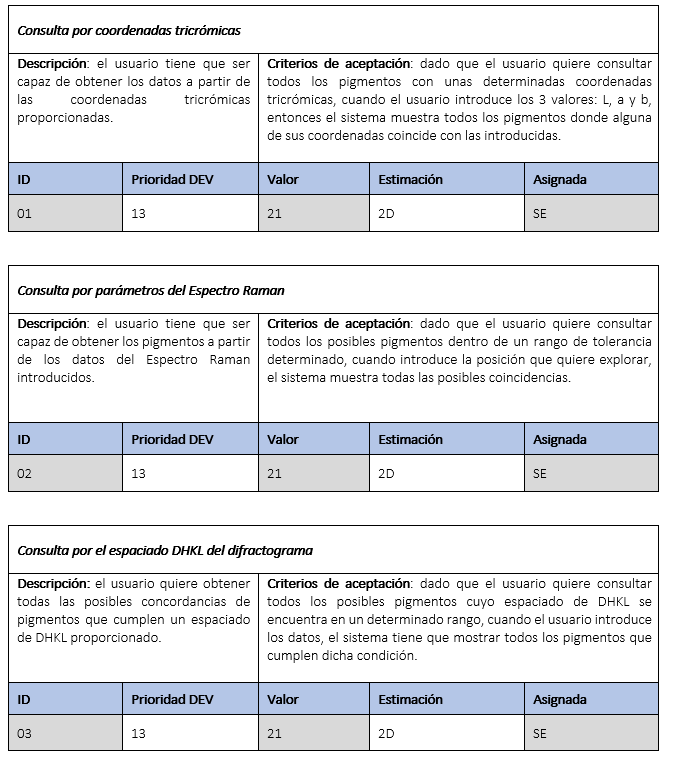
\includegraphics[scale=0.8]{imagenes/diseno/us13.png}
    \label{fig:us13}
\end{figure}

\begin{figure}[H]
    \centering
    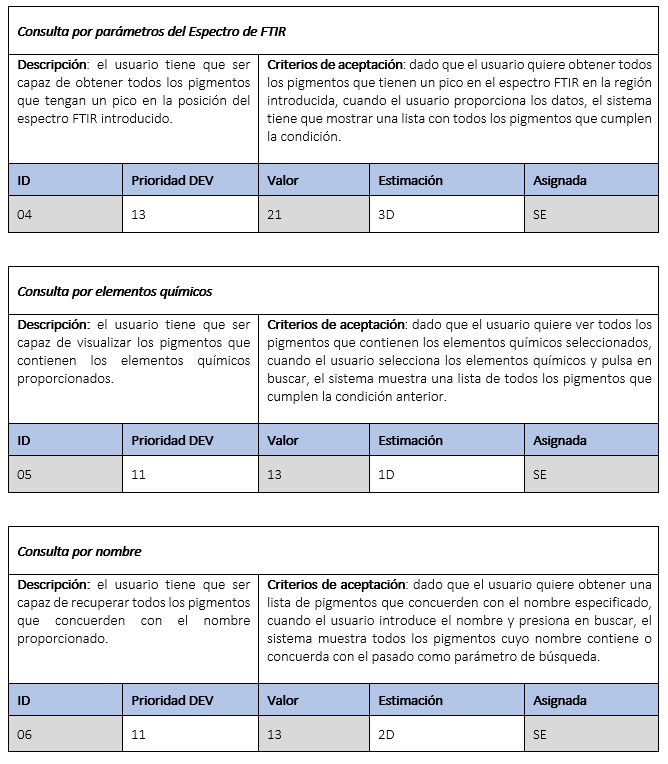
\includegraphics[scale=0.8]{imagenes/diseno/us46.png}
    \label{fig:us46}
\end{figure}

\begin{figure}[H]
    \centering
    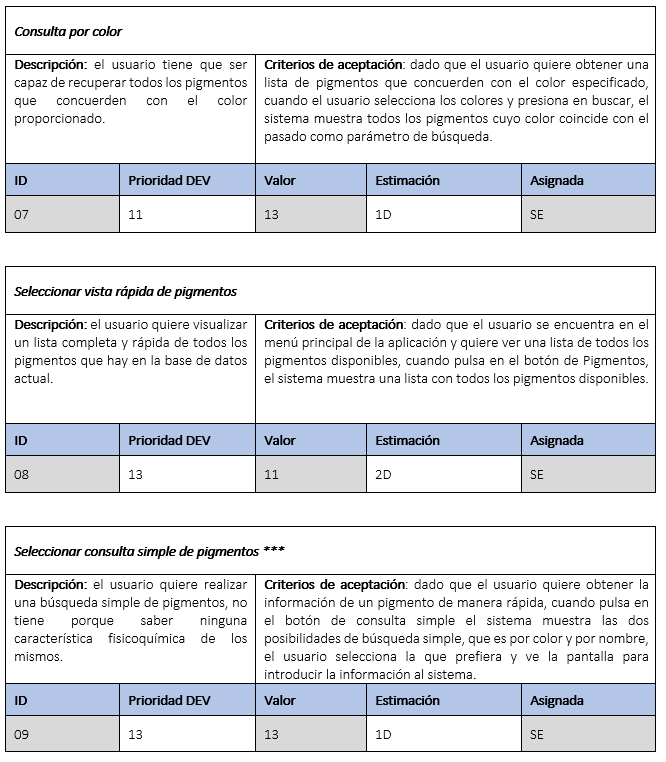
\includegraphics[scale=0.8]{imagenes/diseno/us79.png}
    \label{fig:us79}
\end{figure}

\begin{figure}[H]
    \centering
    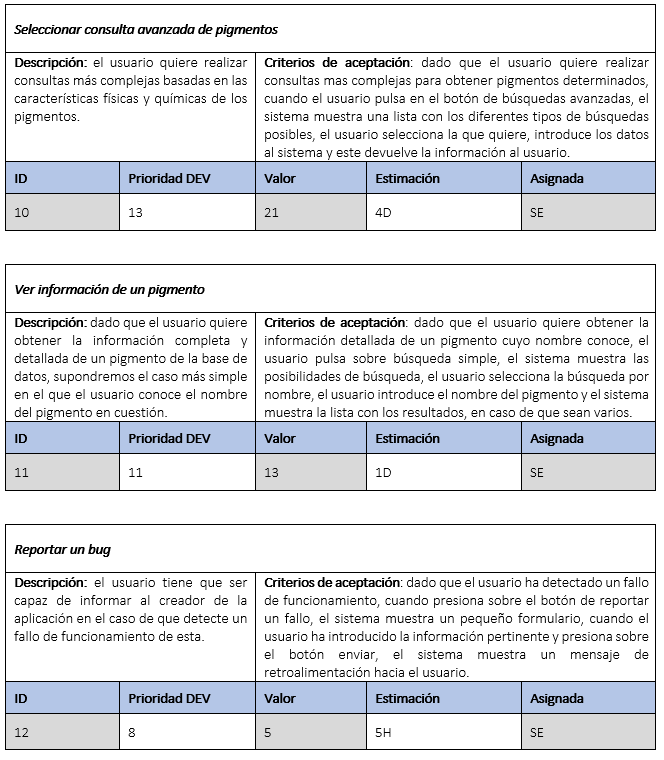
\includegraphics[scale=0.8]{imagenes/diseno/us1012.png}
    \label{fig:us1012}
\end{figure}

\begin{figure}[H]
    \centering
    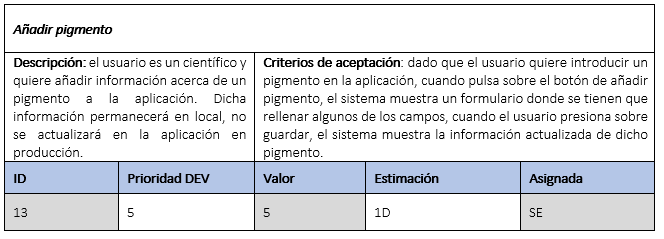
\includegraphics[scale=0.8]{imagenes/diseno/usTrece.png}
    \label{fig:usTrece}
\end{figure}

Ahora que ya tenemos el backlog ordenado, sabemos las tareas que tenemos que desarrollar, como hay que hacerlo y en que orden, podemos pasar a empezar a desarrollar la aplicación y pensar en cosas de más bajo nivel. También podemos observar, que estas historias de usuario tiene diferentes dependencias entre ellas, como es esperable en el desarrollo de una aplicación, por ejemplo podemos completar la parte de las consultas avanzadas si no tenemos el desarrollo de la interfaz principal. 

La precedencia de tareas la podemos observar en la \textbf{Figura \ref{fig:precedenciaTareas}}

\begin{figure}[H]
    \centering
    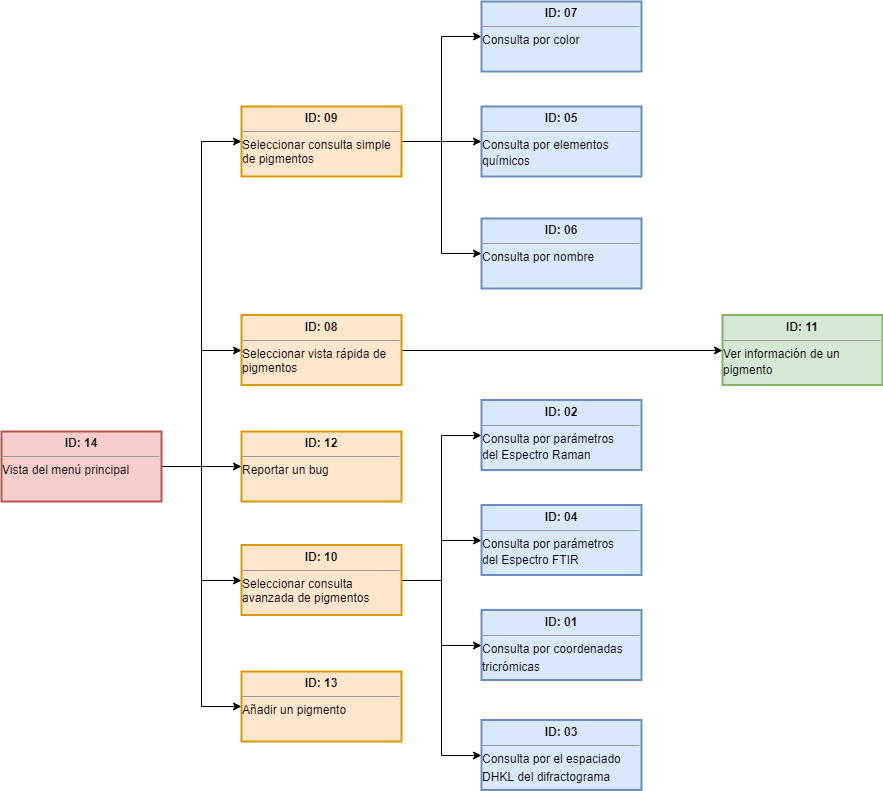
\includegraphics[scale=0.5]{imagenes/diseno/precedenciasTareas.png}
    \caption{Diagrama de precedencia de las principales tareas}
    \label{fig:precedenciaTareas}
\end{figure}

Muchas de las tareas, como la ID:07, ID:05 o ID:02 desembocan también en la ID:11, pero no están relacionadas porque no es estrictamente necesario que todas ellas estén terminadas para poder empezar la 11, la única que si que tiene que estar necesariamente terminada para poder empezar con la ID:11 es la ID:08. 

